\documentclass[12pt]{article}
\usepackage[utf8]{inputenc}
\usepackage[nottoc]{tocbibind}
\usepackage[titletoc,title]{appendix}

\renewcommand*\familydefault{\sfdefault} 

\usepackage{pgfplots}
\pgfplotsset{compat=1.8}
\usepgfplotslibrary{statistics}

\usepackage{listings}

\usepackage[top=1.25in, bottom=1.25in, left=1.25in, right=1.25in]{geometry}


\usepackage{setspace}
%\doublespacing
%TODO single space in publish version
\listfiles
\usepackage{fancyhdr}
\pagestyle{fancy}
\fancyhf{}
\rhead{Bell \thepage}
\lhead{ES6 Precompiler Efficiency}



\usepackage[
backend=biber,
style=mla 
]{biblatex}

\addbibresource{citations.bib}

%\sources{citations.bib}

\title{Efficiency of Generated ES5 Code From BabelJS vs Closure Compiler}

\author{Ethan Bell \\ Ethan M Bell's CodeLump}
\date{\today}


%hack to include abstract

\begin{document}
\maketitle
\begin{abstract}
New features in ECMAScript6 (ES6) are very useful for developers, but are not yet implemented in enough javascript engines/runtimes to be practical to implement while still desiring compatibility. To remedy this, ECMAScript 6 precompilers were created, some of the most popular among these being Babel and Closure. These precompilers transpile ES6 code into the more compatible ES5 code. In this study, the same ES6 code was transpiled using both Babel and Closure into ES5 code, which was then tested for speed through JSPerf. The initial hypothesis that Babel's outputted code is faster was confirmed. It is therefore advisable to use Babel for ECMAScript 6 precompilation until such time as ES6 becomes more widely implemented in javascript engines.
\end{abstract}

\thispagestyle{empty}
\clearpage


\tableofcontents
\thispagestyle{empty}
\clearpage


\setcounter{page}{1}
\setlength{\parindent}{0cm}
\setlength{\parskip}{1em}

\section{Introduction}
\subsection{Purpose}
The purpose of this experiment is to determine which ECMAScript 6 (ES6) precompiler, Babel or Closure, generates the most efficient ECMAScript 5 (ES5) code, as measured by speed of execution in the V8 javascript engine, with V8 being chosen due to its dominance of the javascript execution market \cite{jsstats}. These precompilers allow developers to utilize the new features of ES6 while maintaining the compatibility of ES5, and knowing which is the most efficient will allow these developers' new code to also run relatively fast.
\subsection{Background and Motivation}
ECMAScript, more commonly referred to as JavaScript (JS), is the web-standard scripting language \cite{crockpop}. Used in most websites, javascript provides advanced interactive functionality such as tooltips and animation. The functionality provided by JS to extend webpages' capabilities is incredible; However, due to poor object modeling, its name (a satire of the language Java), and numerous other "quirks", JS has a relatively poor reputation among professional developers \cite{crockpop}.

In order to improve JS and its appeal to developers, the ES6 proposal sets the following goals: improve large application support, support libraries, and make ES6 a more attractive compilation target \cite[xvii]{ecma}. Being a better compilation target means being a better language to run code in. At the moment, JS is not the most pleasant language to use to write and run code \cite{crockpop}, and ES6 aims to fix this. However, the new features of ES6 cannot be run on an ES5 JS engine like V8 (unless the engine is modified to support ES6). Therefore, for greater compatibility, precompilers were produced to take ES6 code and recompile it with the compilation target of ES5. In summary, ES6 code run through a precompiler becomes potentially slower but far more compatible ES5 code. Given that the ES5 code produced is machine-generated, it can have various levels of efficiency. The purpose of this experiment is to test those levels, and to determine which precompiler produces the fastest code.

\subsection{Features to be tested}
The first feature integrated into the ES6 code to be tested for precompilation efficiency was arrow functions. Resembling the notation used in lamda calculus, arrow functions provide a more compact method of expressing and defining functions in a way similar to C\#, CoffeeScript, and other popular languages \cite{hoban}. Given that they are processed almost exactly the same as traditional functions, efficiency of execution should not be too poorly affected by precompilation to ES5, and the resulting code should be relatively simple \cite[86, 249]{ecma}.

Another feature which was tested was destructuring syntax. Destructuring syntax is a compact way of assigning values to sets of variables without breaking apart and then re-combining those sets \cite{hoban}. This feature was used as something of a wildcard, as I couldn't determine the ease of efficient compilation by reviewing the ECMAScript specification. As part of this test, the new "spread" (...) operator was also used, which does something similar in expanding data into a different form that would normally take recombination \cite{hoban}.

%TODO: remove the footnote in publishing version
Lastly, let and const declarations were tested for efficiency. let and const declarations are new methods of defining variables in ES6. let declarations provide more variable security (that is, greater restrictions on access and modification of variables) by restricting variable access to the scope of the block in which the variable is declared \cite{hoban}. const operates in much the same way, with the additional restriction that a value assigned by const is immutable, or constant, meaning it can't be overwritten later \cite{hoban}. The specifics of the functionality of let and const are not really necessary for this experiment, however, just the understanding that ES6 let and const statements work only slightly differently than ES5 variable declarations, yet still differently enough that extra code is necessary for correct functionality.
\subsection{Hypothesis}
Due to its usage in performance-intensive web technology-based applications such as Flipboard, Atom, Netflix, Cloudflare, and Yahoo!, I predicted that Babel will produce the fastest code \cite{babel}. As further support of its more advanced development, Babel supports more ES6 features \cite{compat}.
\section{Methodology}
\subsection{Software Versions and Testing Environment}
\begin{itemize}
\item Windows 8.1 64-bit Build 9600
\item 12GB RAM
\item 14GB virtual memory
\item Intel i7-4710HQ
\item Google Chrome 32-bit Official Build 42.0.2311.135 with flags --javascript-harmony --manual-enhanced-bookmarks
\item jsPerf (http://jsperf.com/)
\item Babel v5.2.15 (http://babeljs.io/)
\item Closure v20150505 (https://github.com/google/closure-compiler/)
\end{itemize}


\subsection{Procedures}
\begin{enumerate}
\item The softwares were downloaded and installed
\item The code (Appendix A) was added to the file \texttt{in.js}
\item The code (Appendix A) was run through closure using the command \texttt{java -jar compiler.jar in.js --language\_in=ECMASCRIPT6 --language\_out=ES5 \\
--js\_output\_file=closureout.js}
\item The code (Appendix A) was run through babel using the command \texttt{babel in.js -o babelout.js}
\item The contents of closureout.js and babelout.js were copied into the "Code snippet 1" and "Code snippet 2" fields of jsPerf, respectively
\item The jsPerf page was generated and assigned the url http://jsperf.com/es6testing
\item The jsPerf tests were run
\item The operations per second data were recorded
\item Steps 7-8 were repeated 14 more times
\end{enumerate}

\section{Results and Discussion}
\subsection{Data}
\begin{tabular}{lll}
Trial & Closure (ops/sec) & Babel (ops/sec) \\
1     & 961,760           & 964,424         \\
2     & 948,241           & 982,245         \\
3     & 959,354           & 983,706         \\
4     & 957,510           & 984,387         \\
5     & 950,520           & 966,674         \\
6     & 942,229           & 959,627         \\
7     & 928,698           & 949,760         \\
8     & 925,528           & 969,058         \\
9     & 927,008           & 938,628         \\
10    & 880,245           & 939,446         \\
11    & 892,422           & 946,013         \\
12    & 957,849           & 999,665         \\
13    & 868,791           & 908,324         \\
14    & 873,249           & 900,882         \\
15    & 861,712           & 884,077        
\end{tabular}
    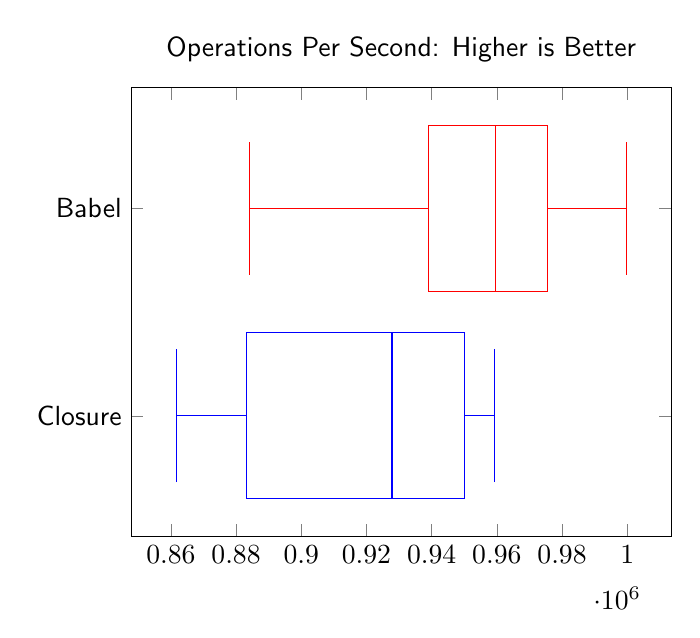
\begin{tikzpicture}
      \begin{axis}
        [
        ytick={1,2},
        yticklabels={Closure, Babel},
        title={Operations Per Second: Higher is Better}%,
        %xlabel={Boxplot. Source: Author}
        ]
        \addplot+[
        boxplot prepared={
          median=927853,
          upper quartile=949950.25,
          lower quartile=883289.25,
          upper whisker=959354,
          lower whisker=861712
        },
        ] coordinates {};
        \addplot+[
        boxplot prepared={
          median=959627,
          upper quartile=975651.5,
          lower quartile=939037,
          upper whisker=999665,
          lower whisker=884077
        },
        ] coordinates {};
      \end{axis}
    \end{tikzpicture}

\subsection{Discussion and Possibilities for Further Research}
As indicated by the box plots, Babel was clearly faster. This finding confirms my hypothesis. Interestingly, the maximum number of operations (ops) per second reached by Closure (959354) wasn't even as much as the median number of ops per second performed by Babel (959,627). This is strange, given that Closure is specifically designed to write efficient code \cite{closure}. Only as an additional feature is it a ES6 precompiler. On the other hand, for the same reason it may make more sense that Babel, designed as an ES6 precompiler, is more efficient when compiling from ES6 \cite{babel}. In any case, further research could be performed into the specific functionality of Babel and Closure, as well as possibly other pre- and transpilers. This would provide a more deductive approach to figuring out what precompiler is the most efficient. One notable discrepancy is Babel's inclusion of the strict mode declaration \texttt{"use strict";} which may affect performance in the V8 engine. However, based on the results of this study, it is advisable to use Babel over Closure for the purposes of ES6 precompilation.


\clearpage
\printbibliography[
heading=bibintoc,
title={Works Cited}
]
\clearpage
\begin{appendices}
\section{Sample ES6 Code}
\lstinputlisting[language=Java,breaklines=true]{in.js}
\clearpage
\section{Closure Compiled ES5 Code}
\lstinputlisting[language=Java,breaklines=true]{closureout.js}
\clearpage
\section{Babel Compiled ES5 Code}
\lstinputlisting[language=Java,breaklines=true]{babelout.js}
\end{appendices}
\end{document}